We ran OTM-MPI simulations on a Cray XC40 Cori supercomputer at NERSC~\cite{Cori}. Each node has two sockets, each socket is
populated with a 16-core Intel\textcopyright~Xeon\texttrademark~Processor E5-2698 v3 (``Haswell'') at 2.3 GHz and 128 GB of RAM memory. This is a very modern parallel computer, taking advantage of recent technology advances in parallel computers.

\subsection{Experiment on Large-scale Synthetic Network}
\begin{figure}[h!]
    \centering
    \includegraphics[height=3in]{figs/Grid-Network.png}
    \caption{Topology of Large-scale Synthetic Network with 62500 nodes and 170,000 links}
    \label{fig:Synthetic_Network}
\end{figure}

We conducted experiments on a large, grid-like, synthetic network, with a topoloty shown in fig. \ref{fig:Synthetic_Network}, to demonstrate the scalability of the parallel OTM in large networks. The network was composed of 62,500 nodes and 170,000 links. The traffic demand was from 12,500 origin destination pairs and the simulation was run for 1000 seconds. Fig. \ref{fig:mpirun} show the bread-down of the time used for loading and configuring the network into OTM format (load), running the simulation (run), and communication between the network partitions, as the number of processes increased from 1 to 1024. As the number of processes used for simulation increased, the size of the network partition per process also decreased. Accordingly, the time to load, simulated and communicate also decreased as each process had less computation/communication to do.

\begin{figure}[h!]
    \centering
    \includegraphics[width=\columnwidth]{figs/mpirun.png}
    \caption{OTM Time Breakdown for Simulating 62,500 Node Grid Network}
    \label{fig:mpirun}
\end{figure}
Fig. \ref{fig:scaling} demonstrate the scaling of parallel OTM compared to the ideal scaling simulation rate. For each simulation experiment, the simulation rate $1/(simulation \:time)$, which corresponds to the number of simulations that can be completed within 1 seconds (simulations/s). The ideal rate is calculated as $(number\: of\: processes)*(serial\: simulation\: rate)$, and assumes that simulation rate increases proportionally with the number of processes. In practice, parallel simulation does not attain the ideal scaling rate as the $(communication\:time)/(simulation\:time)$ ratio grows with the number of processes. In fact, we observed that for the experiment with 1024 processes, each process spend half of its computation time in communicating with other processes. However, we still observed that for the simulation time, the parallel OTM had a speed up of 475 times with 1024 processes compared to the serial OTM. This corresponded to a time reduction from 8,245 seconds to 17 seconds and speed up of 485 times compared to the serial simulation.

\begin{figure}[ht]
    \centering
    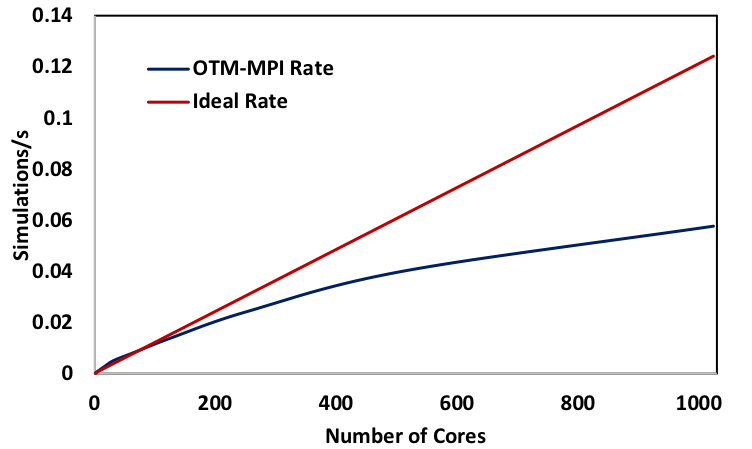
\includegraphics[width=\columnwidth]{figs/Scaling.png}
    \caption{OTM Scaling Rate compared to Ideal Scaling Rate when Simulating Grid Network}
    \label{fig:scaling}
\end{figure}

\subsection{Experiment on Chattanooga Tennessee Network}

\begin{figure}[ht]
    \centering
    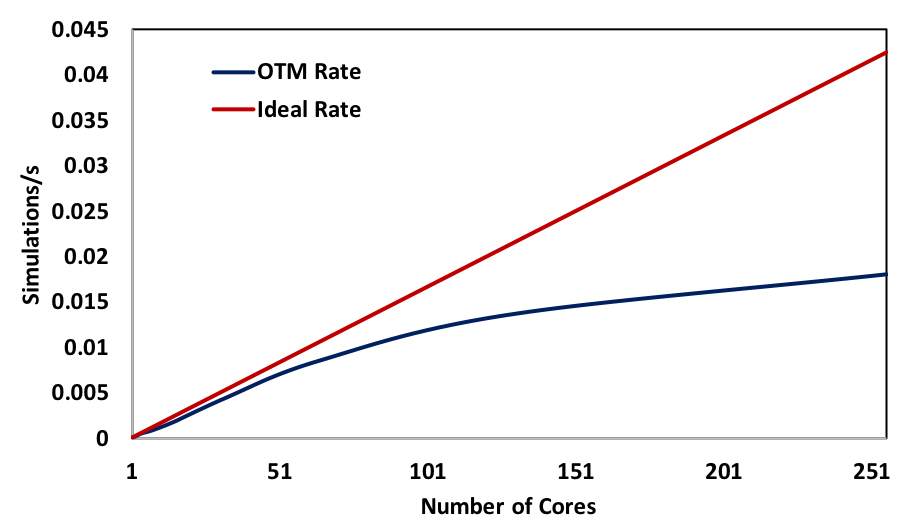
\includegraphics[width=\columnwidth]{figs/Chattanooga_Rate.png}
    \caption{OTM Scaling when simulating the Chattanooga Region}
    \label{fig:ChattanoogaRate}
\end{figure}

We also conducted simulation experiments on a network Chattanooga, Tennessee, region. The goal was to demonstrate how the parallel OTM scale when simulating a large traffic networks with realistic topology. The Chattanooga network had 32260 nodes and 38440 links, and was extracted from OpenStreetMap\cite{haklay2008openstreetmap}. We then converted the network into OTM network format. This scenario had 248 demand sources with an average of 2000 vehicle/hour demand, and was simulated for 10,000 time-steps. 
Figure \ref{fig:Chattanooga_Sim} shows the distribution of time when simulating the Chattanooga region. As previously, the computing amount per core decreases as the number of cores increases, and this leads to a decrease in simulation, communication and network loading time. For this realistic network, parallel computing also reduced the computing time significantly from 6026 seconds with one computer core to 30 seconds with 256 cores, which corresponds to a speed up of 197 times compared to the serial simulation. Figure \ref{fig:ChattanoogaRate} shows the OTM scaling on the Chattanooga network, which is similar to the scaling on the grid synthetic network. 
We also conducted experiments to verify that the parallel OTM maintained the same traffic states as the serial OTM. We did this by comparing the vehicle density in every link and every 100 time-steps between the serial simulation and parallel simulations. 

% Having Issue adding this Graph
% \begin{figure}[ht]
%     \centering
%     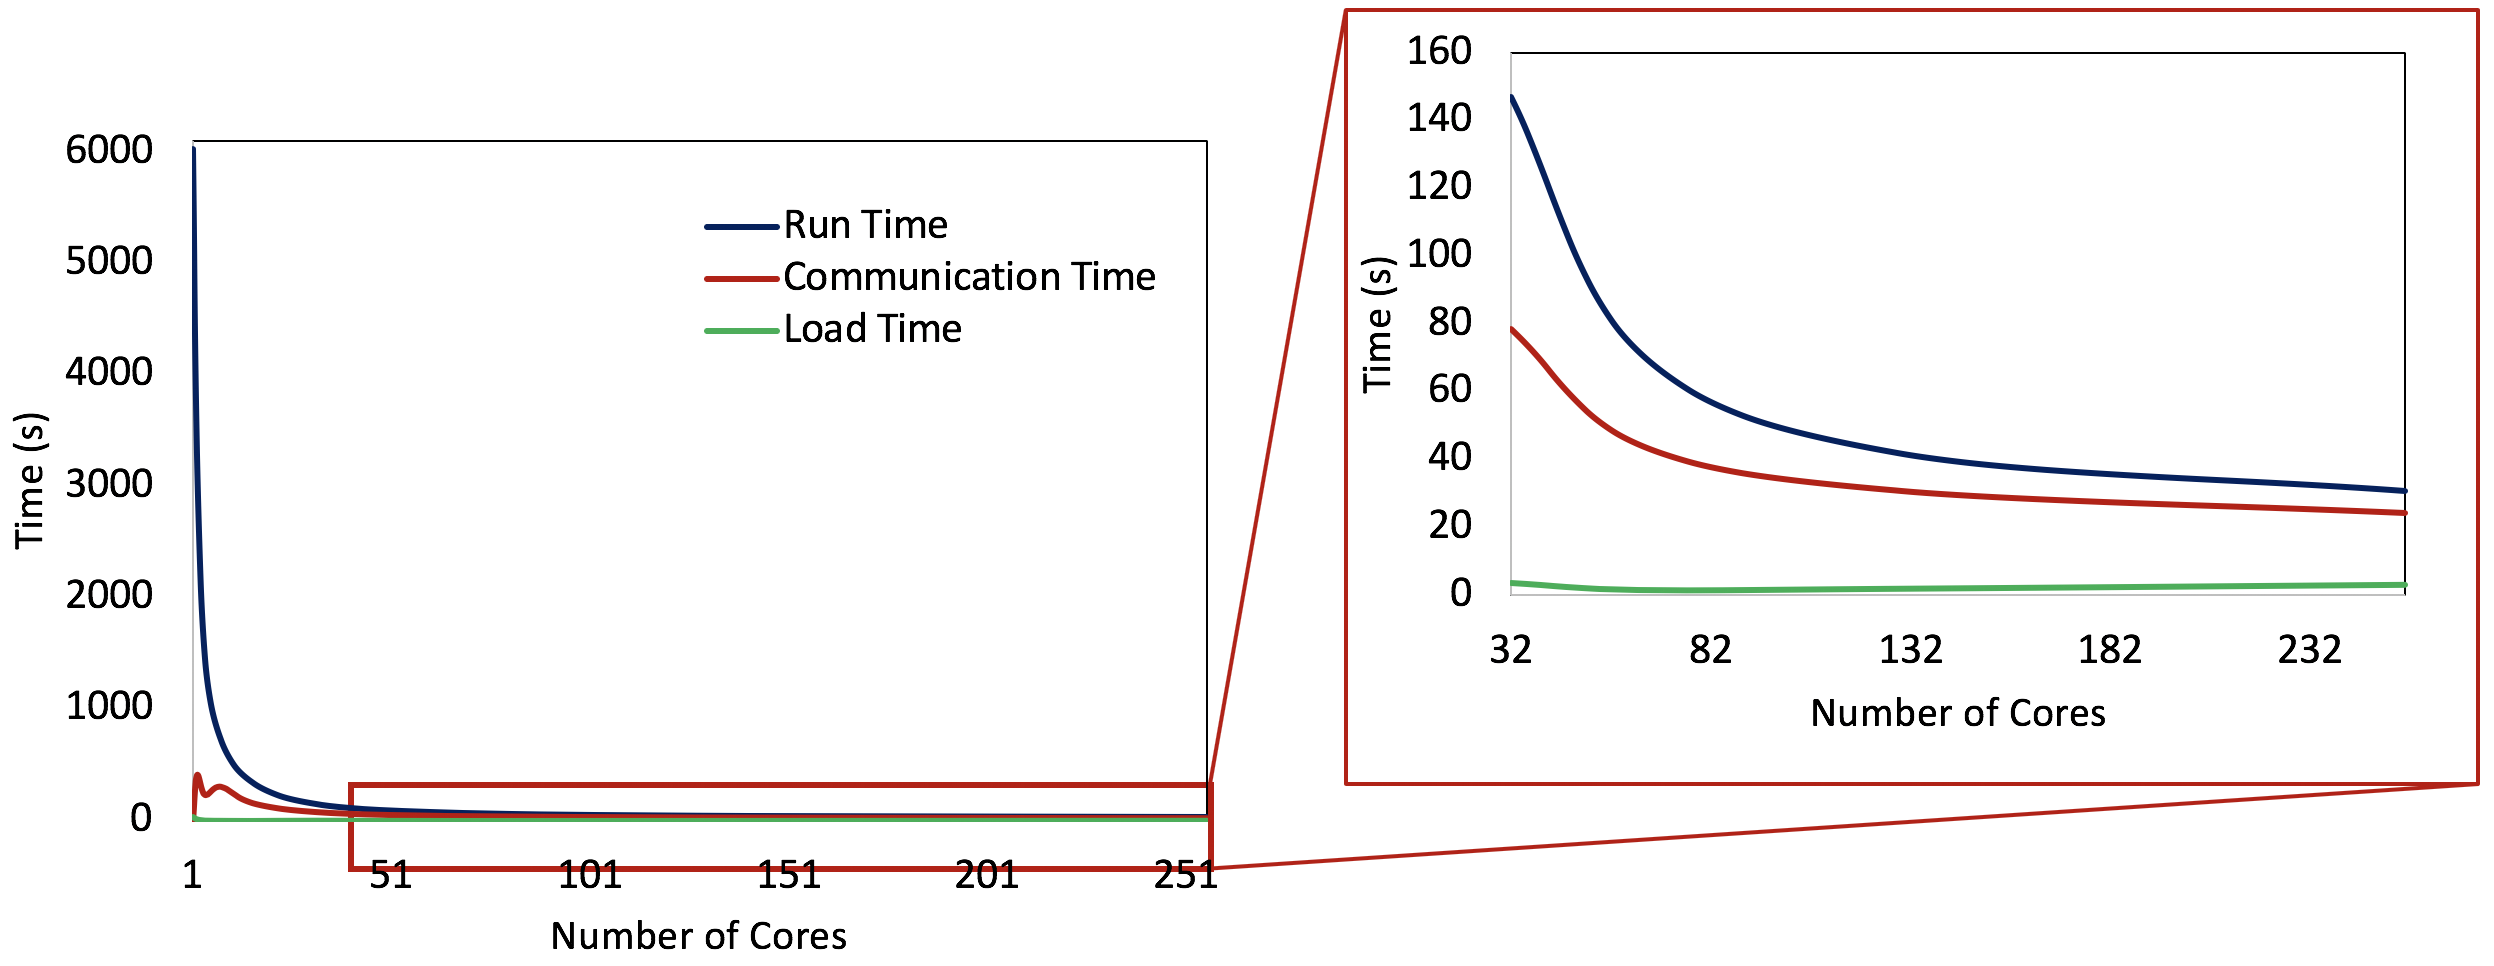
\includegraphics[width=\columnwidth, height=2in]{figs/Chattanooga_Runtime.png}
%     \caption{Distribution of Simulation Time for the Chattanooga Region Network}
%     \label{fig:Chattanooga_Sim}
% \end{figure}

\vspace{1in}



% Network Statistics:
%     88408 nodes
% 	121946 edges



% Figure\ref{fig:chicago}


% \begin{figure}[h!]
%     \centering
%     \includegraphics[height=3in]{figs/Chicago_Net_Black_White.png}
%     \caption{CAPTION.}
%     \label{fig:chicago}
% \end{figure}
 








% \subsection{Extra-Projection Method}
% The Extra-Projection method is an algorithm used to solve the dynamic user equilibrium problem. The inputs to the problem are a traffic network and a set of traffic demand $d_w : [0,T]\rightarrow \mathbb{R}^+ $, where $w\in\mathcal{W}$ is the set of origin destinations (OD) pairs. A solution $h$ is vector of demand on all available $ p\in\mathcal{P}$, where $h_p$ is the demand on path $p$. An optimal solution is a solution that creates a Wardrop traffic equilibrium \cite{wardrop1952some}. 

% EPM is based on the Euclidean projection defined as $\Pi_\mathcal{H}(x) = \underset{h}{\text{argmin}}\{\lvert h-x\rvert_2 \; : \;h \in\mathcal{H} \}$ and convergences when the travel cost function $F$ is Lipschitz continuous and pseudo-monotone. EMP has the following steps \cite{nie2010solving}:
% \begin{enumerate}
%     \item Start with an initial feasible solution $h^{1}$, set $k=1$ and set $\tau^1$ to a value less than the Lipschitz constant of $F$
%     \item Stop if $\frac {\langle c^k,y^k-h^k \rangle}{\langle y^k, c^k\rangle} \leq \epsilon$, where $c^k$ is a vector of travel cost $c_p^k$ for each path  $ p\in\mathcal{P}$ given demand $h^k$ and $y^k$ is the all-or-nothing assignment.
%     \item Determine $h^{k+1} = \Pi_\mathcal{H}(h^k - \tau^k F(z^k))$, and go back to step (2).
% \end{enumerate}

% The most time-consuming steps of the above algorithm are step 2 when calculating the all-or-nothing assignment, and steps 3 and 4 when performing the projection. This is because they involve looping over all the OD pairs, to determine the shortest path in step 2 and euclidean projection for step 3 and 4. Given $N$ computing cores, parallel computation is used to distribute the $\mathcal{W}$ od pairs among the $N$ cores such that each compute core performs step 2, 3 and 4 for $\mathcal{W}/N$ od pairs. 
